\documentclass{article}
\usepackage[utf8]{inputenc}
\usepackage[spanish]{babel}
\usepackage{amsmath}
\usepackage{amssymb}
\usepackage{amsfonts}
\usepackage{hyperref}
\usepackage{textcomp}
\usepackage{graphicx}
\usepackage{pgfplots}
\usepackage{geometry}
\hypersetup{
    colorlinks=true,
    linkcolor=black,
    citecolor=green,
    filecolor=magenta,      
    urlcolor=cyan,
}
\geometry{
  top=3cm,            % Margen superior
  bottom=3cm,         % Margen inferior
  left=3cm,           % Margen izquierdo
  right=3cm           % Margen derecho
}

\title{Estadística 1}
\author{Jorge Miguel Alvarado Reyes}
\date{16 Agosto 2023}

\setlength{\parindent}{0pt}
\begin{document}

\begin{titlepage}
    \begin{center}
        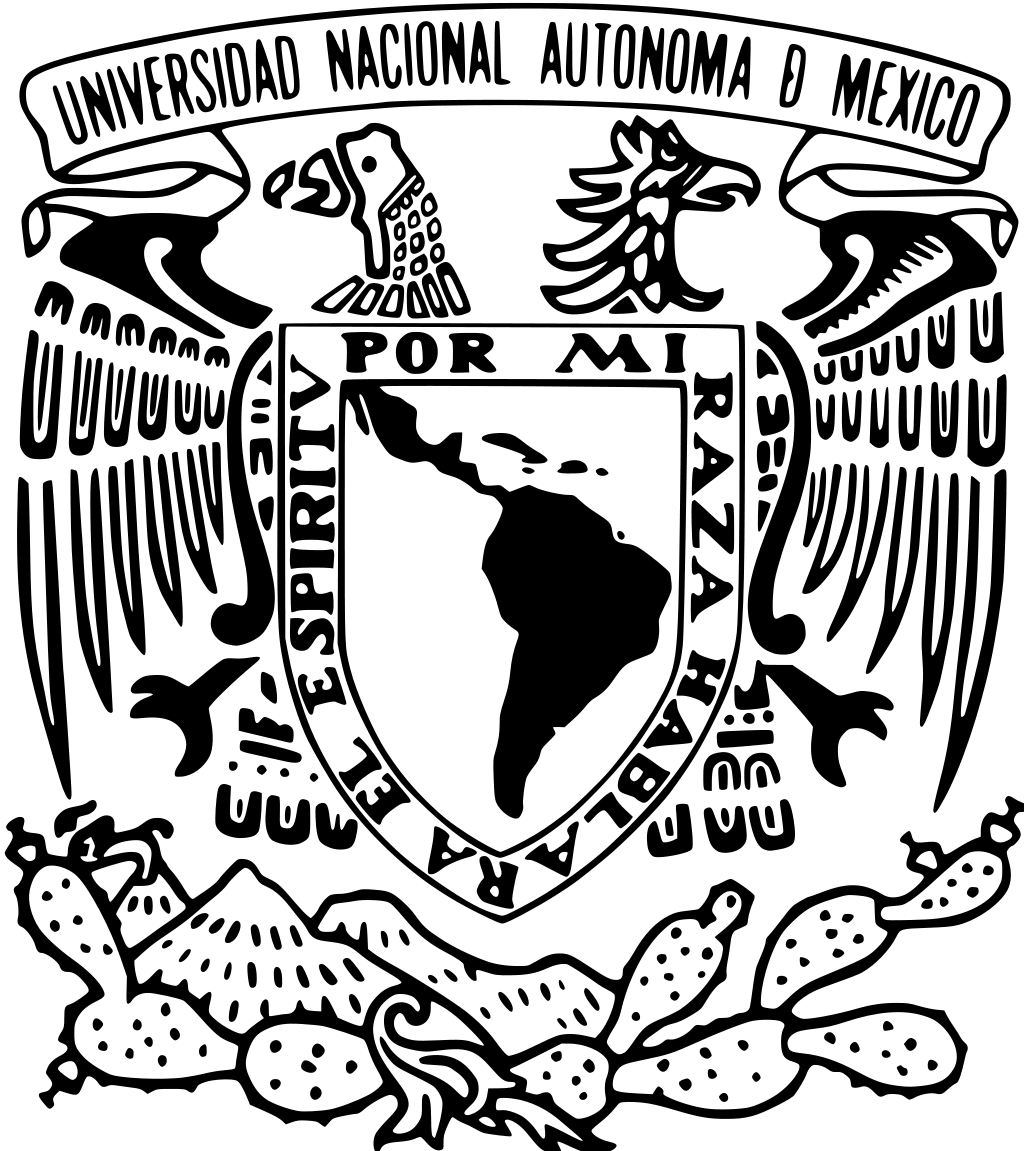
\includegraphics[width=0.2\textwidth]{../../unam.png}
        \vspace*{.5cm}

        \LARGE
        \textbf{Universidad Nacional Autónoma de México}

        \vspace{0.5cm}
        \LARGE
        Facultad de Estudios Superiores Acatlán

        \vspace{2cm}

        \textbf{Apuntes} \\
        Procesos Estocasticos

        \vfill

        \vspace{1cm}

        \textbf{\large Autor:} \\
        Jorge Miguel Alvarado Reyes \\
        \vspace{.5cm}
        \normalsize \today

    \end{center}
\end{titlepage}
\newpage

\tableofcontents

\newpage

\section{Problema 1}

Demuestre que para un $N_n$ definido en un proceso de Bernoulli, la varianza, $\text{Var}(N_n)$, es igual a $npq$
Sea \( X \) el número de éxitos, entonces:
\[ E(N_n) = np \]

Para cualquier \( X_i \):
\[ P(X_i = 1) = p \text{ Exito}\]
\[ P(X_i = 0) = 1 - p = q \text{ Fracaso}\]

Entonces la esperanza de \( X \) es:
\[ E(N_n) = E(X_1) + E(X_2) + \ldots + E(X_n) \]

Para cualquier \( X_i \):
\[ E(X_i) = 0 \cdot q + 1 \cdot p = p \]

Entonces:
\[ E(N_n) = p + p + p \text{ Asi n veces}\]
\[ E(N_n) = np\]

ahora debemos encontrar $E(N_n^2)$

\[E(N_n^2) = \sum_{k=0}^{n} k^2 \cdot P(N_n = k)\]

\[P(N_n = k) = \binom{n}{k} p^k q^{n-k}\]

entonces

\[E(N_n^2) = \sum_{k=0}^{n} \binom{n}{k} p^k q^{n-k}\]

\[E(N_n^2) = npq + (np)^2\]

Entonces la varianza es

\[Var(N_n) = E(N_n^2) - E(N_n)^2\]

\[Var(N_n) = npq + (np)^2 - (np)^2\]

\[Var(N_n) = npq\]

\section{Problema 2}

Demuestre que la funcion generatriz de momentos de la caminata aleatoria es $M(t) = (pe^t + qe^{-t}) * n$. Recuerda que la funcion generatriz de momentos es: $m(t) = E(e^{tx})$


\subsection*{Paso 1: Definición de la Función Generatriz de Momentos}
La función generatriz de momentos $m(t)$ de una variable aleatoria $X$ se define como:
\[ m(t) = E[e^{tX}] \]

\subsection*{Paso 2: Aplicación a la Caminata Aleatoria}
Para un solo paso $X_i$ de la caminata, donde $X_i = +1$ con probabilidad $p$ y $X_i = -1$ con probabilidad $q$, la función generatriz de momentos es:
\[ m_i(t) = E[e^{tX_i}] = pe^{t(+1)} + qe^{t(-1)} = pe^t + qe^{-t} \]

\subsection*{Paso 3: Función Generatriz de Momentos para $n$ Pasos}
Considerando que la caminata aleatoria está compuesta por $n$ pasos independientes y que la función generatriz de momentos para la suma de variables aleatorias independientes es el producto de sus funciones generatriz de momentos individuales, la función generatriz de momentos para la caminata aleatoria completa, $M(t)$, es:
\[ M(t) = (m_i(t))^n = (pe^t + qe^{-t})^n \]


\section{Problema 3}

Demuestre que para $n,k \in \{1,2,3,\dots\}$

\[P\{N_{n+1} = k\} = p * P\{N_n = k-1\} + q * P\{N_n = k\}\]

donde $N_n$ es el número de éxitos en $n$ ensayos de Bernoulli, $p$ es la probabilidad de éxito, y $q = 1 - p$ es la probabilidad de fracaso.

Utilizando la ley de probabilidad total:
\[ P\{N_{n+1} = k\} = P\{N_{n+1} = k | N_n = k-1\} \cdot P\{N_n = k-1\} + P\{N_{n+1} = k | N_n = k\} \cdot P\{N_n = k\} \]

En un ensayo solo puede ocurrir un éxito o un fracaso:
\[ P\{N_{n+1} = k | N_n = k-1\} = p \]
\[ P\{N_{n+1} = k | N_n = k\} = q \]

La fórmula se reduce a:
\[ P\{N_{n+1} = k\} = p \cdot P\{N_n = k-1\} + q \cdot P\{N_n = k\} \]

\section{Problema 4}

Demuestre la formula de probabilidades de transicion de una caminata alaeatoria simple usando ahora los pasos que se dan a la izquierda

\section{Problema 5}

Para una caminata aleatoria simple \(X_n\) sobre los enteros, demuestre que:
\[ P(X_{n+1} = x) = pP(X_n = x - 1) + qP(X_n = x + 1) \]

Sugerencia: Sustituya los parámetros de las probabilidades en la fórmula de probabilidades de transición de una caminata aleatoria y con álgebra verifique la igualdad.

\section{Problema 6}

Una partícula realiza una caminata aleatoria simétrica sobre los enteros empezando en 0. Encuentre la probabilidad de que la partícula no se encuentre nuevamente en el origen en el sexto paso.

\section{Practica 2}

\subsection*{Problema 1}

Considere que existe una partícula que realiza una caminata aleatoria sobre los números enteros, iniciando en 3. La probabilidad de dar un paso a la derecha es de \( \frac{2}{3} \). Encuentre la probabilidad de que la partícula se encuentre:

\begin{enumerate}
    \item[a)] En la posición 8 en 10 pasos.
    \item[b)] Regrese a la posición 3 en 6 pasos.
\end{enumerate}

\subsubsection*{Punto a}

La probabilidad de que la partícula se encuentre en la posición 8 después de 10 pasos es:
\[
    P\{X_{10} = 8 | X_0 = 3\} = \binom{10}{\frac{10 + 8 - 3}{2}} \left(\frac{2}{3}\right)^{\frac{10 + 8 - 3}{2}} \left(\frac{1}{3}\right)^{\frac{10 - 8 + 3}{2}},
\]
dado que \( \frac{10 + 8 - 3}{2} \) no es un número entero, la probabilidad es 0. esto se debe a que no se puede llegar a una posicion par dando un numero par de pasos desde una posicion inicial impar

\subsubsection*{Punto b}

La probabilidad de que la partícula regrese a la posición 3 en 6 pasos es:
\[
    P\{X_6 = 3 | X_0 = 3\} = \binom{6}{\frac{6 + 3 - 3}{2}} \left(\frac{2}{3}\right)^{\frac{6 + 3 - 3}{2}} \left(\frac{1}{3}\right)^{\frac{6 - 3 + 3}{2}},
\]
aplicando los valores obtenemos que la probabilidad es aproximadamente 0.2195 o 21.95\%.

\subsection*{Problema 2}

Considere una partícula que realiza una caminata aleatoria simple simétrica sobre los enteros. Encuentre la probabilidad de que la partícula se encuentre:

\begin{enumerate}
    \item[a)] En la posición 5 en 9 pasos.
    \item[b)] En la posicion 3 o 7 en 10 pasos
    \item[c)] En la posicion 2 en 7 pasos
\end{enumerate}

\subsubsection*{Punto a}


La probabilidad de que la partícula se encuentre en la posición 5 después de 9 pasos, comenzando desde una posición inicial \(X_0\), es:
\[
    P\{X_9 = 5 | X_0 = X_0\} = \binom{9}{7} \left(\frac{1}{2}\right)^{7} \left(\frac{1}{2}\right)^{2},
\]

\[
    P\{X_9 = 5 | X_0 = X_0\} = \binom{9}{7} \left(\frac{1}{2}\right)^{9},
\]

\[
    P\{X_9 = 5 | X_0 = X_0\} = 0.0703125,
\]
lo que representa una probabilidad del 7.03125\%.

\subsubsection*{Punto b}

No es posible llegar a una posicion impar danndo un numero par de pasos

\subsubsection*{Punto c}

No es posible llegar a una posicion par dando un numero impar de pasos

\section{Cadena de markov}

\subsection{Problema 1}

Considere el modelo del valor de una acción. Al final de un día dado se registra el precio. Si la acción subió la probabilidad de que suba mañana es de 0.7. Si la acción bajó, la probabilidad de que suba mañana es de sólo 0.5. (Por simplicidad, cuando una acción permanezca con el mismo valor, se considerará un aumento)

El \textbf{espacio de estados} \( S \) es definido como:

\[ S = \{ \text{Sube}, \text{Baja} \} \]

Donde:
\begin{itemize}
    \item "Sube" indica que el precio de la acción sube o permanece igual (considerado como aumento).
    \item "Baja" indica que el precio de la acción baja.
\end{itemize}

% Matriz de Transición
La \textbf{matriz de transición} \( P \) representa las probabilidades de pasar de un estado a otro. Para este modelo, la matriz es:
\[ P = \begin{pmatrix} 0.7 & 0.3 \\ 0.5 & 0.5 \end{pmatrix} \]

Donde:
\begin{itemize}
    \item La primera fila \( \begin{pmatrix} 0.7 & 0.3 \end{pmatrix} \) representa las probabilidades de transición desde el estado "Sube": Si hoy el precio subió (o se mantuvo igual), la probabilidad de que suba mañana es de 0.7 y la de que baje es de 0.3.
    \item La segunda fila \( \begin{pmatrix} 0.5 & 0.5 \end{pmatrix} \) representa las probabilidades de transición desde el estado "Baja": Si hoy el precio bajó, la probabilidad de que suba mañana es de 0.5 y la de que baje es también de 0.5.
\end{itemize}

\subsection{Problema 2}

Suponga ahora que el modelo de mercado de acciones se cambia de manera que el hecho de que una acción suba o no mañana, depende de si subió o no hoy y ayer. En particular, si la acción subió los dos días, ayer y hoy, la probabilidad de que suba mañana es de 0.9. Si la acción subió hoy, pero ayer bajó, la probabilidad de que mañana suba es de 0.6. Si la acción bajó hoy pero ayer subió la probabilidad de que mañana suba es de 0.5. Si bajó durante estos 2 días, la probabilidad de que mañana suba es de 0.3.

Considere solo 4 estados, SUBIÓ-SUBIÓ, SUBIÓ-BAJÓ, BAJÓ-SUBIÓ, BAJÓ-BAJÓ.

\[S={SUBIO-SUBIO,SUBIO-BAJO,BAJO-SUBIO,BAJO-BAJO}\]

\[
    P = \begin{bmatrix}
        0.9 & 0.1 & 0   & 0   \\
        0   & 0   & 0.6 & 0.4 \\
        0.5 & 0.5 & 0   & 0   \\
        0   & 0   & 0.3 & 0.7 \\
    \end{bmatrix}
\]

\subsection{Problema 3}

La compañía Colgate ha estado promoviendo un nuevo tipo de detergente. El resultado de dicha promoción es que el 75\% de las personas que usan el detergente durante un período de un mes continúan utilizándolo. De las personas que usan otro detergente durante un período de un mes, un 45\% cambia al detergente de Colgate al mes siguiente.


Definimos el \textbf{espacio de estados} \( S \) como:
\[ S = \{ \text{Colgate}, \text{Otro} \} \]

La \textbf{matriz de transición} \( P \) es:
\[ P = \begin{pmatrix}
        0.75 & 0.25 \\
        0.45 & 0.55 \\
    \end{pmatrix} \]

\end{document}